\documentclass[t, pdftex]{beamer}  
%Use Cockrell School Theme.  Optional department name.  Must %ecape, i.e. use 
%backslash, to preserve spaces.  The default is ``Cockrell School of Engineering''
%\usetheme[]{Cockrell}                 
%\usetheme[dept=Aerospace\ Engineering\ and\ Engineering\ Mechanics]{cockrell}                 
%\usetheme[dept=Biomedical\ Engineering]{cockrell}                 
%\usetheme[dept=Chemical\ Engineering]{cockrell}                 
%\usetheme[dept=Civil,\ Architectural\ and\ Environmental\ Engineering]{cockrell}                 
\usetheme[dept=Electrical\ and\ Computer\ Engineering]{Cockrell}                 
%\usetheme[dept=Mechanical\ Engineering]{cockrell}                 
%\usetheme[dept=Materials\ Science\ and\ Engineering]{cockrell}                 
%\usetheme[dept=Petroleum\ and\ Geosystems\ Engineering]{cockrell}                 

% Add preamble packages here
%\usepackage{etex}
%\usepackage[bigfiles]{media9}
\usepackage{graphicx}
\graphicspath{{../figs/}}
\usepackage{caption}

\usepackage{listings,multicol}
\definecolor{ForestGreen}{rgb}{0.13,0.55,0.13}
\lstset{
    language         = Promela,
    basicstyle       = \ttfamily,
    keywordstyle     = \bfseries\color{blue},
    stringstyle      = \color{magenta},
    commentstyle     = \color{ForestGreen},
    showstringspaces = false,
}

%Enable cancelto in math
\usepackage{cancel}
\renewcommand{\CancelColor}{\color{utorange}}

%Add bibliography file location for citiation
% \bibliography{example.bib}


\title{Verifying Distributed Algorithms}
\subtitle{in Promela}
\author{Eric Crosson \\ Nhan Do \\ Stormy Mauldin \\ Daniel Officewala}
\institute{EE 360P}
\date{\today}


\begin{document}

%Creates title frame from title, subtitle, author, institute, and date above
\titleframe

%Supports table of contents
\frame{\frametitle{Outline}\tableofcontents}

%Section commands will define what's shown in TOC

%First frame
\section{Introducing Promela}
\begin{frame}
    \frametitle{Cockrell School Beamer Presentation Template}

    \begin{itemize}
        %Support for external hyperlinks as shown
        \item Conforms to \href{http://www.engr.utexas.edu/communications/visualguidelines}{Cockrell School Visual Style Guide}
        \begin{itemize}
            \item Exact color palette
            \item Opensans fonts
        \end{itemize}
        \item Easily change department names in title bar
        %Citations can use \footcite or \cite commands
        % \item Convenient citation system \footcite{knuth1989} \cite{lamport1986}
        \begin{itemize}
            \item Full citation with active hyperlinks to DOI upon first citation.
            \item See next slide for repeated citation behavior
        \end{itemize}
    \end{itemize}
\end{frame}

\section{Dining Philosophers}
\begin{frame}[c]
    \frametitle{Dining Philosophers}
    % \TeX\ \cite{knuth1989} and \LaTeX\ \cite{lamport1986} are great for equations
    \begin{block}{An equation block}
        \[ \vec{F} = m \vec{a} \]
    \end{block}
    \begin{itemize}
        \item Second instance of citations use short citation hyperlinked to original.
    \end{itemize}
\end{frame}

\section{Token Ring}
\begin{frame}[c]
    \frametitle{Token Ring Algorithm}
    % \TeX\ \cite{knuth1989} and \LaTeX\ \cite{lamport1986} are great for equations
    \begin{itemize}
		\item Simple and easily scalable
		 \begin{itemize}
          \item Pass token around ring of processes
          \item Only processes with token can enter CS
		  \item No Starvation
        \end{itemize}
    \end{itemize}
	
	
 \begin{figure}
	 \begin{minipage}{.5\textwidth}
      \centering
      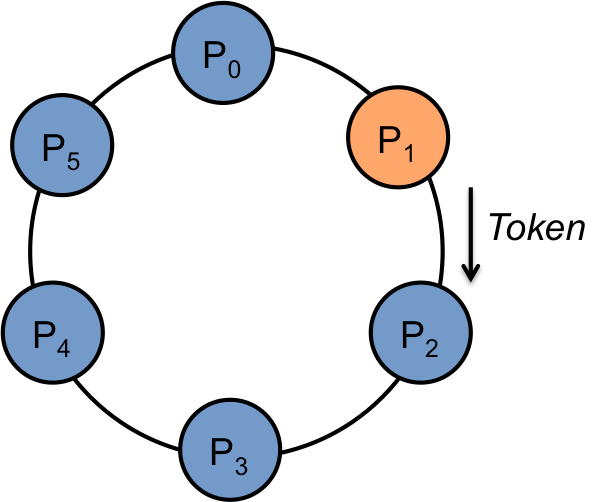
\includegraphics[scale=.30]{tokenring}
      \captionof{figure}{Token Ring Algorithm}
      \label{fig:Token Ring}
    \end{minipage}
\end{figure}
	
\end{frame}

\begin{frame}
	\frametitle{Token Ring Implementation}
	  \begin{multicols*}{3}
    \lstinputlisting[language=Promela, basicstyle=\tiny]{../figs/tokenring.pml}
  \end{multicols*}
\end{frame}



\section{Lamport's}
\begin{frame}[c]
    \frametitle{Lamport's}
    % \TeX\ \cite{knuth1989} and \LaTeX\ \cite{lamport1986} are great for equations
    \begin{block}{An equation block}
        \[ \vec{F} = m \vec{a} \]
    \end{block}
    \begin{itemize}
        \item Second instance of citations use short citation hyperlinked to original.
    \end{itemize}
\end{frame}

\section{Szymanski's}
\begin{frame}[c]
    \frametitle{Szymanski's Algorithm}
    \begin{itemize}
      \item Extension of Lamport's
        \begin{itemize}
          \item satisfies linear wait
          \item three booleans per process
        \end{itemize}
      \item Extension of Lamport's
    \end{itemize}
  % PRO POINTS: make your own charts here, don't be a scrub
  \begin{figure}
    \centering
    \begin{minipage}{.5\textwidth}
      \centering
      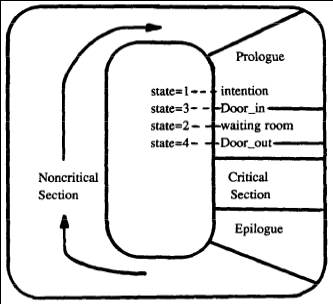
\includegraphics[scale=.3]{szymanskis_carosel}
      \captionof{figure}{Szymanski's Algorithm}
      \label{fig:szymanskis_carosel}
    \end{minipage}%
    \begin{minipage}{.5\textwidth}
      \centering
      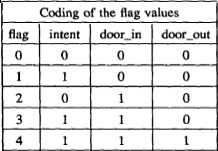
\includegraphics[scale=.61]{szymanskis_booleans}
      \captionof{figure}{State-tracking booleans}
      \label{fig:szymanskis_booleans}
    \end{minipage}
  \end{figure}
\end{frame}

\begin{frame}
  \frametitle{Szymanski's Implementation}
  \begin{multicols*}{3}
    \lstinputlisting[language=Promela, basicstyle=\tiny]{../figs/szymanski.pml}
  \end{multicols*}
\end{frame}

\begin{frame}
  \frametitle{Szymanski's Analysis}
  
\end{frame}

\section{Questions}
\begin{frame}[c]
    \frametitle{Questions}  % verbally, say ``What are your questions?'' 
    % \TeX\ \cite{knuth1989} and \LaTeX\ \cite{lamport1986} are great for equations
    \begin{itemize}
        \item English mothafucka, do you speak it?
    \end{itemize}
\end{frame}


% This command is causing problems
% I am not sure what we're missing out on by not having it.
%\lastframe%
\end{document}
